\documentclass[../../../../main.tex]{subfiles}

\begin{document}

\section*{第1問}

\begin{proof}[解]
図のように$\theta$をおく。又，$a_n$個の円の中心を$O_1\sim O_n$とする。半径1の円の中心を$O$として，図から，
\[
\sin\theta=\frac{\frac1n}{1+\frac1n}=\frac{1}{n+1} \quad \cdots \text{①}
\]

\begin{center}
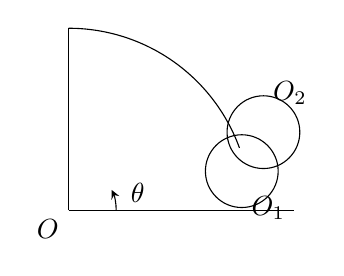
\begin{tikzpicture}[scale=1.1, >=stealth]
  \draw (0,0) -- (0,2.1);
  \draw (0,0) -- (2.6,0);
  \draw[domain=90:20,smooth] plot ({2.1*cos(\x)},{2.1*sin(\x)});
  \draw[->] (0.55,0) arc (0:25:0.55);
  \node at (0.8,0.2) {$\theta$};
  \node[below left] at (0,0) {$O$};
  \draw (2.0,0.45) circle (0.42);
  \draw (2.25,0.9) circle (0.42);
  \node[right] at (2.0,0.02) {$O_1$};
  \node[right] at (2.25,1.35) {$O_2$};
\end{tikzpicture}
\end{center}

又，題意から
\[
2a_n\cdot\theta\le2\pi<2(a_n+1)\theta
\]
\[
\frac{\pi}{n\theta}-\frac1n\le\frac{a_n}{n}<\frac{\pi}{n\theta} \quad \cdots \text{②}\ (\because n>0)
\]
ここで①から$n\to\infty$の時$\theta\to0$で，これと①から
\[
\frac{1}{n\theta}=\frac{1}{n\sin\theta}\cdot\frac{\sin\theta}{\theta}=\frac{n+1}{n}\cdot\frac{\sin\theta}{\theta}=\frac{1+\frac1n}{1}\cdot\frac{\sin\theta}{\theta}\longrightarrow1 \quad(n\to\infty)
\]
だから②とはさみうちから
\[
\frac{a_n}{n}\longrightarrow\pi
\]
\end{proof}

\newpage

\section*{第2問}

\begin{proof}[解]
$\vec a,\vec b$のなす角$\theta$とおく。この時対称性から，$0<\theta\le\dfrac{\pi}{2}\ \cdots$①で考えれば良い。この時，$\cos\theta\ge0$から
\[
|\vec a\pm\vec b|=\sqrt{2\pm2\cos\theta} \quad \cdots *
\]
より，$|\vec a+\vec b|>|\vec a-\vec b|$となることに注意する。

\begin{enumerate}
  \item[(1)] 対称性から，$m\ge0$で示せば良い。$m=0$から明らかに$\min L=1$だから，以下$m>0$とする。
  \[
  |L|^2=m^2+n^2+2mn\cos\theta \quad \cdots \text{①}
  \]
  であり，これは$m,n$について単調増加だから，$n\ge0$の時は$(m,n)=(0,1)$の時$\min L=1$，$n\le0$の時は$(m,n)=(1,0)$の時$\min L=1$である（0ベクトルのぞいた） $\cdots$②

  次に$n<0$の時，$n'=-n$とおくと，$n'>0$となり，①から
  \[
  |L|^2=m^2+n'^2-2mn'\cos\theta=(m-n')^2+2mn'(1-\cos\theta)\ge2(1-\cos\theta)\quad(\text{等号成立は}\ m=n'=1,\ \because m>0,n'>0)
  \]
  \[
  =|\vec a-\vec b|^2
  \]
  だから，たしかに$(m,n)=(1,-1)$で$\min L=|\vec a-\vec b|$をとる。 $\cdots$③

  ②③から，$0<\theta\le\dfrac{\pi}{2}$の時$r=1$ or $|\vec a-\vec b|$である。$\dfrac{\pi}{2}\le\theta<\pi$の時は対称性から$r=1$ or $|\vec a+\vec b|$となる。以上から示された。

  \item[(2)] 引き続き①のもとで考える。すから，条件は
  \[
  |\vec a-\vec b|\ge1 \iff 2-2\cos\theta\ge1 \iff \frac{\pi}{3}\le\theta\le\frac{\pi}{2} \quad \cdots \text{④}
  \]
  だから$S=\dfrac12\sin\theta$の$\min$は，$\theta=\dfrac{\pi}{3}$の時の$\dfrac{\sqrt3}{4}$である。
\end{enumerate}
\end{proof}

\bigskip
\noindent\textbf{[解2]}

\begin{proof}[解]
$m\ge0$，$0<\theta\le\dfrac{\pi}{2}$とする。斜行座標を考える。図のように半径2の円を描くと，$(m,n)=(1,\pm1),(1,0),(0,\pm1)$のみが円の内部にあるから，最小値の候補はこれらだけである。よって示された。
\end{proof}

\newpage

\section*{第3問}

\begin{proof}[解]
$C: y=f(x)=x^4-6x^2$とおく。$f'(x)=4x^3-12x$より，$x=t$における$C$の接線$\ell$は
\[
\ell: y=(4t^3-12t)x-3t^4+6t^2
\]
これが$P$を通る時，
\[
\beta=(4t^3-12t)\alpha-3t^4+6t^2 \quad \cdots \text{①}
\]
$C$の2重接線は$y=-9$だけであるから，①が$t$に関して4実解を持てば良い。そこで，$g(t)=3t^4-4\alpha t^3-6t^2+12\alpha t+\beta$とおく。
\[
g'(t)=12t^3-12\alpha t^2-12t+12\alpha=12(t-\alpha)(t+1)(t-1)
\]
より，$\alpha$において下表を得る。まず，$t=0$が解でないので$\beta\ne0$。

\begin{center}
\begin{tabular}{c|ccccccc}
$t$ & & $\alpha$ & & $-1$ & & $1$ & \\
\hline
$g'$ & $-$ & $0$ & $+$ & $0$ & $-$ & $0$ & $+$ \\
\hline
$g$ & $\searrow$ & & $\nearrow$ & & $\searrow$ & & $\nearrow$
\end{tabular}
\quad ($1^\circ\ \alpha\le-1$)
\end{center}
条件は $g(\alpha)<0,\ g(1)<0,\ g(-1)>0$

\begin{center}
\begin{tabular}{c|ccccccc}
$t$ & & $-1$ & & $\alpha$ & & $1$ & \\
\hline
$g'$ & $-$ & $0$ & $+$ & $0$ & $-$ & $0$ & $+$ \\
\hline
$g$ & $\searrow$ & & $\nearrow$ & & $\searrow$ & & $\nearrow$
\end{tabular}
\quad ($2^\circ\ -1\le\alpha\le1$)
\end{center}
条件は $g(-1)<0,\ g(1)<0,\ g(\alpha)>0$

\begin{center}
\begin{tabular}{c|ccccccc}
$t$ & & $-1$ & & $1$ & & $\alpha$ & \\
\hline
$g'$ & $-$ & $0$ & $+$ & $0$ & $-$ & $0$ & $+$ \\
\hline
$g$ & $\searrow$ & & $\nearrow$ & & $\searrow$ & & $\nearrow$
\end{tabular}
\quad ($3^\circ\ 1\le\alpha$)
\end{center}
条件は $g(-1)<0,\ g(\alpha)<0,\ g(1)>0$

ここで
\[
g(1)=\beta+8\alpha-3,\qquad g(-1)=\beta-8\alpha-3,\qquad g(\alpha)=-\alpha^4+6\alpha^2+\beta
\]
である。$g(\alpha)=\beta-f(\alpha)$であり，$P$は$y>x^4-6x^2$の領域にあるから，常に$g(\alpha)>0$である。よって$1^\circ,3^\circ$（$g(\alpha)<0$を要求する）は起こりえず，$2^\circ$（$-1\le\alpha\le1$）のみが可能で，条件は$g(\alpha)>0$が自動的にみたされることから
\[
g(-1)<0\ \text{かつ}\ g(1)<0 \iff \beta<3-8\alpha\ \text{かつ}\ \beta<3+8\alpha
\]
に帰着する。以上から，もとめる領域$D$は
\[
D=\left\{(\alpha,\beta)\ \middle|\ -1<\alpha<1,\ \ \alpha^4-6\alpha^2<\beta<3-8|\alpha|\right\}
\]
であり，図示すると下図（境界含まず）。

\begin{center}
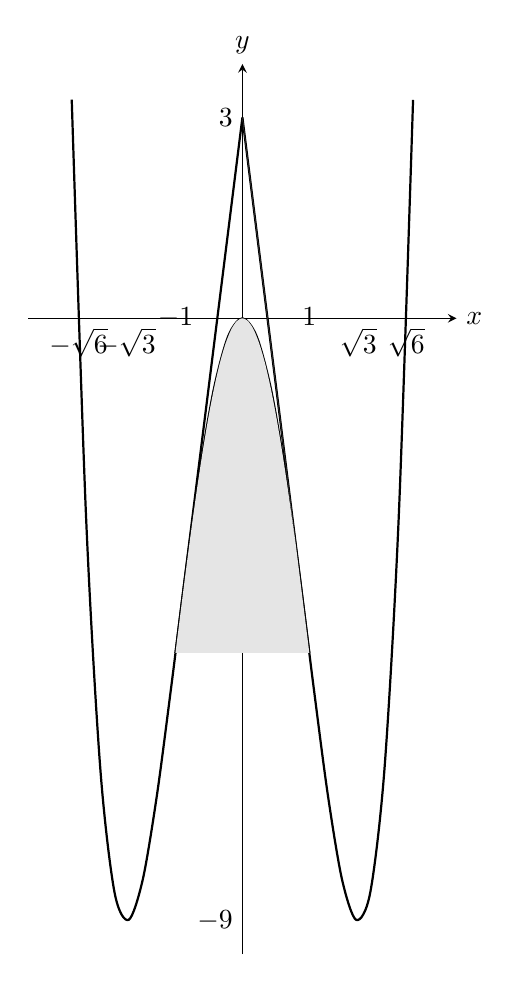
\begin{tikzpicture}[scale=0.85, >=stealth]
  \draw[->] (-3.2,0) -- (3.2,0) node[right] {$x$};
  \draw[->] (0,-9.5) -- (0,3.8) node[above] {$y$};
  \draw[domain=-2.55:2.55, smooth, thick] plot (\x,{\x*\x*\x*\x-6*\x*\x});
  \draw[thick] (0,3) -- (1,-5);
  \draw[thick] (0,3) -- (-1,-5);
  \fill[gray!20] (0,3) -- (1,-5) plot[domain=1:-1,smooth] (\x,{\x*\x*\x*\x-6*\x*\x}) -- cycle;
  \node[left] at (0,3) {$3$};
  \node[below] at (-2.449,0) {$-\sqrt6$};
  \node[below] at (-1.732,0) {$-\sqrt3$};
  \node[below] at (-1,0.3) {$-1$};
  \node[below] at (1,0.3) {$1$};
  \node[below] at (1.732,0) {$\sqrt3$};
  \node[below] at (2.449,0) {$\sqrt6$};
  \node[left] at (0,-9) {$-9$};
\end{tikzpicture}
\end{center}
\end{proof}

\newpage

\section*{第4問}

\begin{proof}[解]
もとの楕円を$\theta$だけ回転させた図形上の点$(X,Y)$とすると
\[
x+yi=(X+Yi)\left(\frac{\sqrt2}{2}-\frac{\sqrt2}{2}i\right)=\frac{\sqrt2}{2}(X+Y)+\frac{\sqrt2}{2}i(-X+Y)
\]
から
\[
(x,y)=\left(\frac{\sqrt2}{2}(X+Y),\ \frac{\sqrt2}{2}(X-Y)\right)
\]
とすれば，
\[
\frac{(X+Y)^2}{12}\cdot\frac12+\frac12\cdot\frac{(X-Y)^2}{4}\le1
\]
である。したがって斜線の部分の概形は下図。
\[
\text{扇型}\ OCD=\frac12\cdot\frac{\pi}{4}\cdot(2\sqrt3)^2=\frac32\pi \quad \cdots \text{①}
\]
又，$\triangle OBC$について，$X=\dfrac{x}{2\sqrt3},\ Y=\dfrac{y}{2}$なる変換をすれば下図斜線部の領域式（単位円）になるので，
\[
\triangle OBC=\frac12\cdot\frac{\pi}{3}\times2\sqrt3\cdot2=\frac{2}{3}\sqrt3\pi \quad \cdots \text{②}
\]
①②から，もとめる面積$S$として
\[
S=\frac32\pi+\frac23\sqrt3\pi=\left(\frac32+\frac{2\sqrt3}{3}\right)\pi
\]

\begin{center}
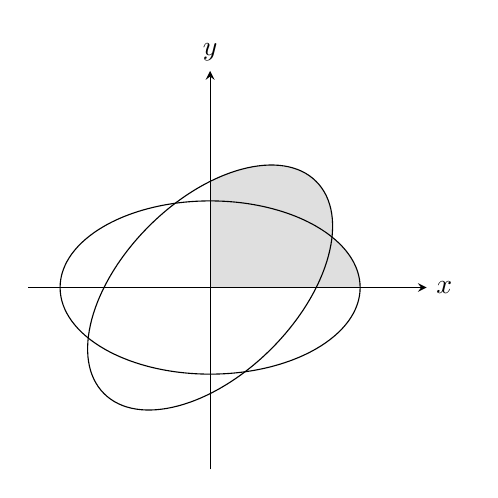
\begin{tikzpicture}[scale=0.55, >=stealth]
  \begin{scope}
    \clip (0,0) rectangle (6,6);
    \fill[gray!25] (0,0) ellipse ({2*sqrt(3)} and 2);
    \begin{scope}[rotate=45]
      \fill[gray!25] (0,0) ellipse ({2*sqrt(3)} and 2);
    \end{scope}
  \end{scope}
  \draw (0,0) ellipse ({2*sqrt(3)} and 2);
  \begin{scope}[rotate=45]
    \draw (0,0) ellipse ({2*sqrt(3)} and 2);
  \end{scope}
  \draw[->] (-4.2,0) -- (5,0) node[right] {$x$};
  \draw[->] (0,-4.2) -- (0,5) node[above] {$y$};
\end{tikzpicture}
\end{center}
\end{proof}

\newpage

\section*{第5問}

\begin{proof}[解]
9つの数の平均の小数第1位が1になるのは，9つの数の和$A$が
\[
1,\ 10\ \text{の時}\quad(0\le A\le18)
\]

\textbf{$A=1$の時}

1回だけ，他が0の時で，
\[
9\left(\frac13\right)^9=\left(\frac13\right)^7
\]

\textbf{$A=10$の時}

\begin{center}
\begin{tabular}{c|c|c|c}
$2$の個数 & $1$の個数 & $0$の個数 & \\
\hline
$5$ & $0$ & $4$ & \\
$4$ & $2$ & $3$ & \\
$3$ & $4$ & $2$ & \\
$2$ & $6$ & $1$ & \\
$1$ & $8$ & $0$ &
\end{tabular}
\end{center}
上表から，
\[
\frac{{}_9C_5+{}_9C_4\cdot{}_5C_2+{}_9C_3\cdot{}_6C_4+{}_9C_2\cdot{}_7C_6+{}_9C_1}{3^9}
\]
\[
=\left(\frac13\right)^9(126+1260+1260+252+9)=\left(\frac13\right)^9\cdot2907=\left(\frac13\right)^7\cdot323
\]
以上から
\[
\left(\frac13\right)^7\cdot324=\frac{4}{3^3}=\frac{4}{27}
\]
\end{proof}

\end{document}
